\documentclass[11pt,a4paper]{article}

\usepackage[margin=1in]{geometry}
\usepackage{booktabs}
\usepackage{array}
\usepackage{longtable}
\usepackage{graphicx}
\usepackage{hyperref}
\usepackage{xcolor}
\usepackage{enumitem}
\usepackage{amsmath}
\usepackage{amssymb}
\usepackage{float}

\hypersetup{
  colorlinks=true,
  linkcolor=blue,
  urlcolor=blue
}

\graphicspath{{figures/}}
\setlist[itemize]{noitemsep, topsep=0.25em}
\emergencystretch=3em

\title{E-Commerce Shopper Behavior Analysis and Prediction Report}
\author{Team 6\\[0.5em]
Nesma Osama -- 9220912\\
Mohamed Ashraf -- 9220658\\
Mazen Adel -- 9220625\\
Mohamed Khater -- 9220713}
\date{\today}

\begin{document}
\maketitle
\tableofcontents
\newpage

\section{Executive Summary}

This project studies e-commerce shopper behavior using the Amazon/Shopify-based shopper behavior dataset. The main prediction target is \texttt{cart\_abandonment\_rate}, which measures how often a shopper leaves a cart without completing a purchase. The project supports both:
\begin{itemize}
  \item a regression task, where the model predicts the continuous cart abandonment rate;
  \item a classification task, where the rate is converted into three ordered classes.
\end{itemize}

The full workflow includes data loading, exploratory analysis, train/validation/test splitting, visualization, feature selection, preprocessing, model training, shopper segmentation, and deployment. The strongest classification models reached about 86\% validation/test accuracy, with Random Forest and Decision Tree slightly ahead of the custom MapReduce ordinal logistic regression.

\section{Problem Description}

Cart abandonment is a major challenge for online retail platforms. A high abandonment rate means that users browse products, add items to the cart, and then leave before completing checkout. This can reduce revenue and expose friction in the shopping experience.

The goal of this project is to identify behavioral, financial, demographic, and psychological signals that explain cart abandonment. The analysis can help an e-commerce platform target promotions, improve recommendations, reduce checkout friction, and segment shoppers into useful behavioral groups.

\section{Dataset}

The source dataset is the Kaggle dataset \textit{E-Commerce Shopper Behavior (Amazon/Shopify Based)}. The original dataset contains one million rows and around sixty columns. Each row describes one shopper using demographic attributes, lifestyle attributes, shopping behavior, platform usage, advertising interaction, and payment preferences.

Important columns include:
\begin{itemize}
  \item cart abandonment rate, the target variable;
  \item monthly spend, cart item average, and purchase conversion rate;
  \item impulse buying score, financial decision stress, and overall stress level;
  \item categorical fields such as device type, education level, budgeting style, and preferred payment method.
\end{itemize}

The project removes identifiers and date fields that are not used directly by the models:
\begin{verbatim}
user_id, last_purchase_date
\end{verbatim}

\section{Target Construction}

\subsection{Regression Target}

For regression, the target remains the original continuous value:
\[
y = \texttt{cart\_abandonment\_rate}.
\]

This value is standardized with \texttt{StandardScaler} before linear regression training.

\subsection{Classification Target}

For classification, the target is converted into three ordered classes:
\begin{center}
\begin{tabular}{cl}
\toprule
Class & Meaning \\
\midrule
0 & Low cart abandonment, rate $< 30$ \\
1 & Medium cart abandonment, $30 \leq$ rate $< 60$ \\
2 & High cart abandonment, rate $\geq 60$ \\
\bottomrule
\end{tabular}
\end{center}

The mapping is implemented in the preprocessing notebook as:
\begin{verbatim}
def classify_cart_abandonment(rate):
    if rate < 30:
        return 0
    elif rate < 60:
        return 1
    else:
        return 2
\end{verbatim}

These classes are ordered, so class 2 is higher than class 1, and class 1 is higher than class 0. This is why the custom logistic regression model uses ordinal threshold classifiers.

\section{Data Split}

The dataset is split with a fixed random seed for reproducibility:
\begin{itemize}
  \item 80\% training data;
  \item 10\% validation data;
  \item 10\% test data.
\end{itemize}

The split is performed before feature selection and preprocessing. This prevents validation and test data from influencing training-time transformations.

\section{Exploratory Visualization}

The preprocessing notebook generates categorical plots, numerical plots, and correlation heatmaps. The script \texttt{docs/generate\_preprocessing\_plots.py} recreates these figures from the original CSV when available. If the CSV is not present, it extracts the saved plot outputs embedded in \texttt{preprocessing.ipynb}, which keeps the report build reproducible inside this repository.

\subsection{Categorical Features}

For each categorical feature, the notebook visualizes:
\begin{itemize}
  \item category frequency;
  \item cart abandonment rate by category;
  \item classified cart abandonment count by category.
\end{itemize}

\begin{figure}[H]
\centering
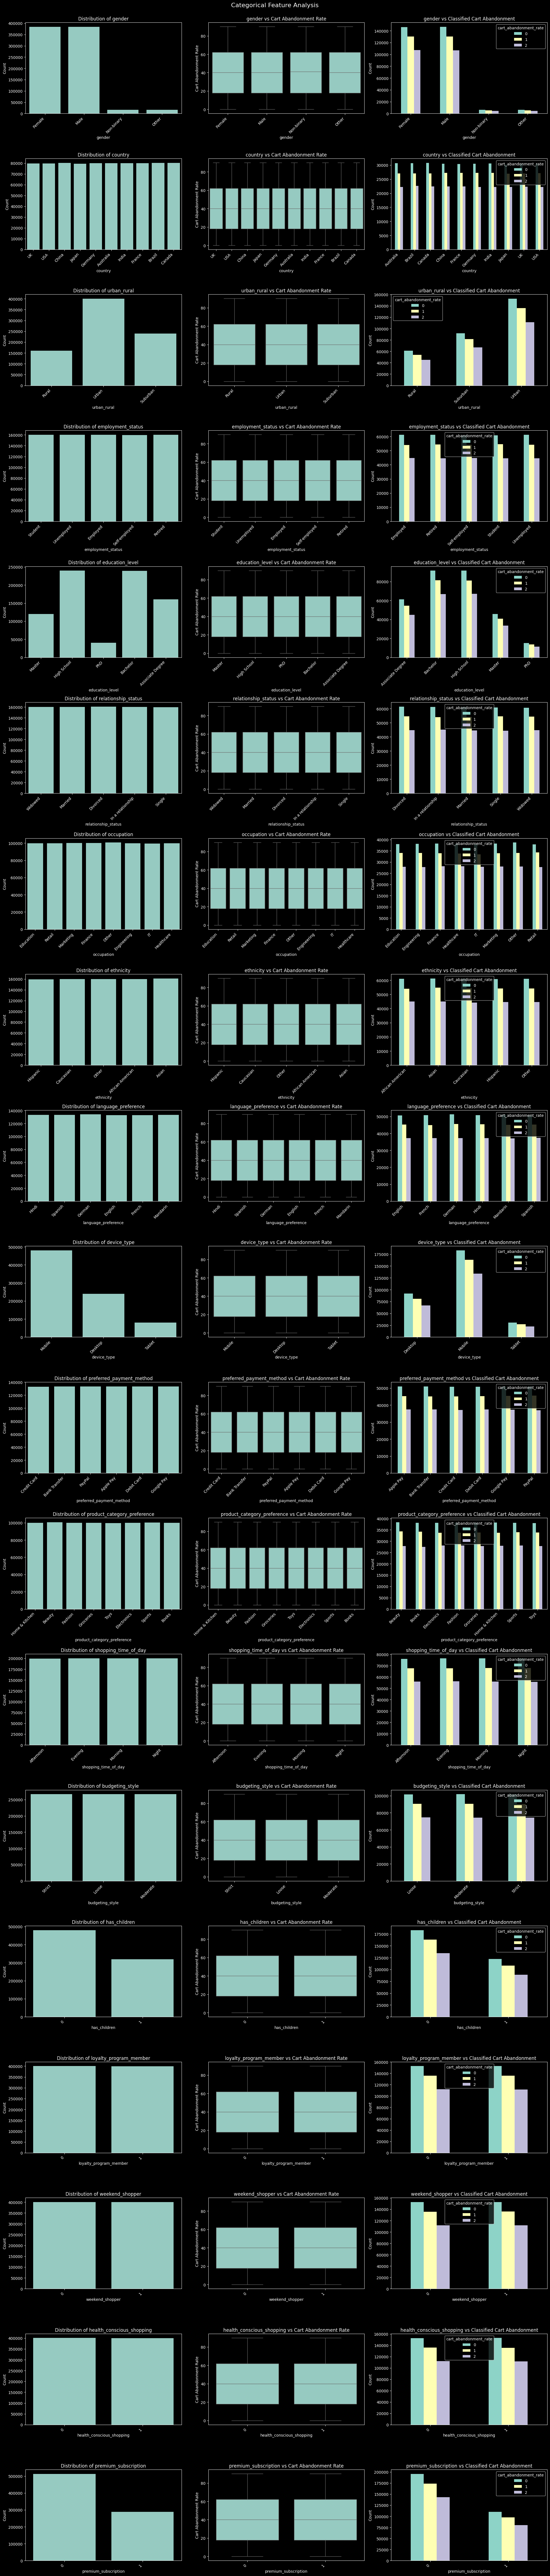
\includegraphics[width=\textwidth,height=0.82\textheight,keepaspectratio]{01_categorical_feature_analysis.png}
\caption{Categorical feature analysis from the preprocessing notebook.}
\end{figure}

The main observations were:
\begin{itemize}
  \item shoppers without children appear more frequently than shoppers with children;
  \item mobile devices appear more frequently than other device types;
  \item High School and Bachelor education levels appear more frequently than other education levels;
  \item non-premium shoppers appear more frequently than premium subscribers;
  \item the class distribution follows class 0, then class 1, then class 2.
\end{itemize}

\subsection{Numerical Features}

For numerical features, the notebook visualizes:
\begin{itemize}
  \item feature distribution with boxplots;
  \item relationship between feature value and continuous cart abandonment rate;
  \item feature distribution across the three classified abandonment classes.
\end{itemize}

\begin{figure}[H]
\centering

\includegraphics[width=\textwidth,height=0.82\textheight,keepaspectratio]{02_numerical_feature_analysis.png}
\caption{Numerical feature analysis from the preprocessing notebook.}
\end{figure}

\subsection{Correlation Analysis}

The full numerical correlation matrix is used to detect redundant features and relationships between behavioral variables.

\begin{figure}[H]
\centering
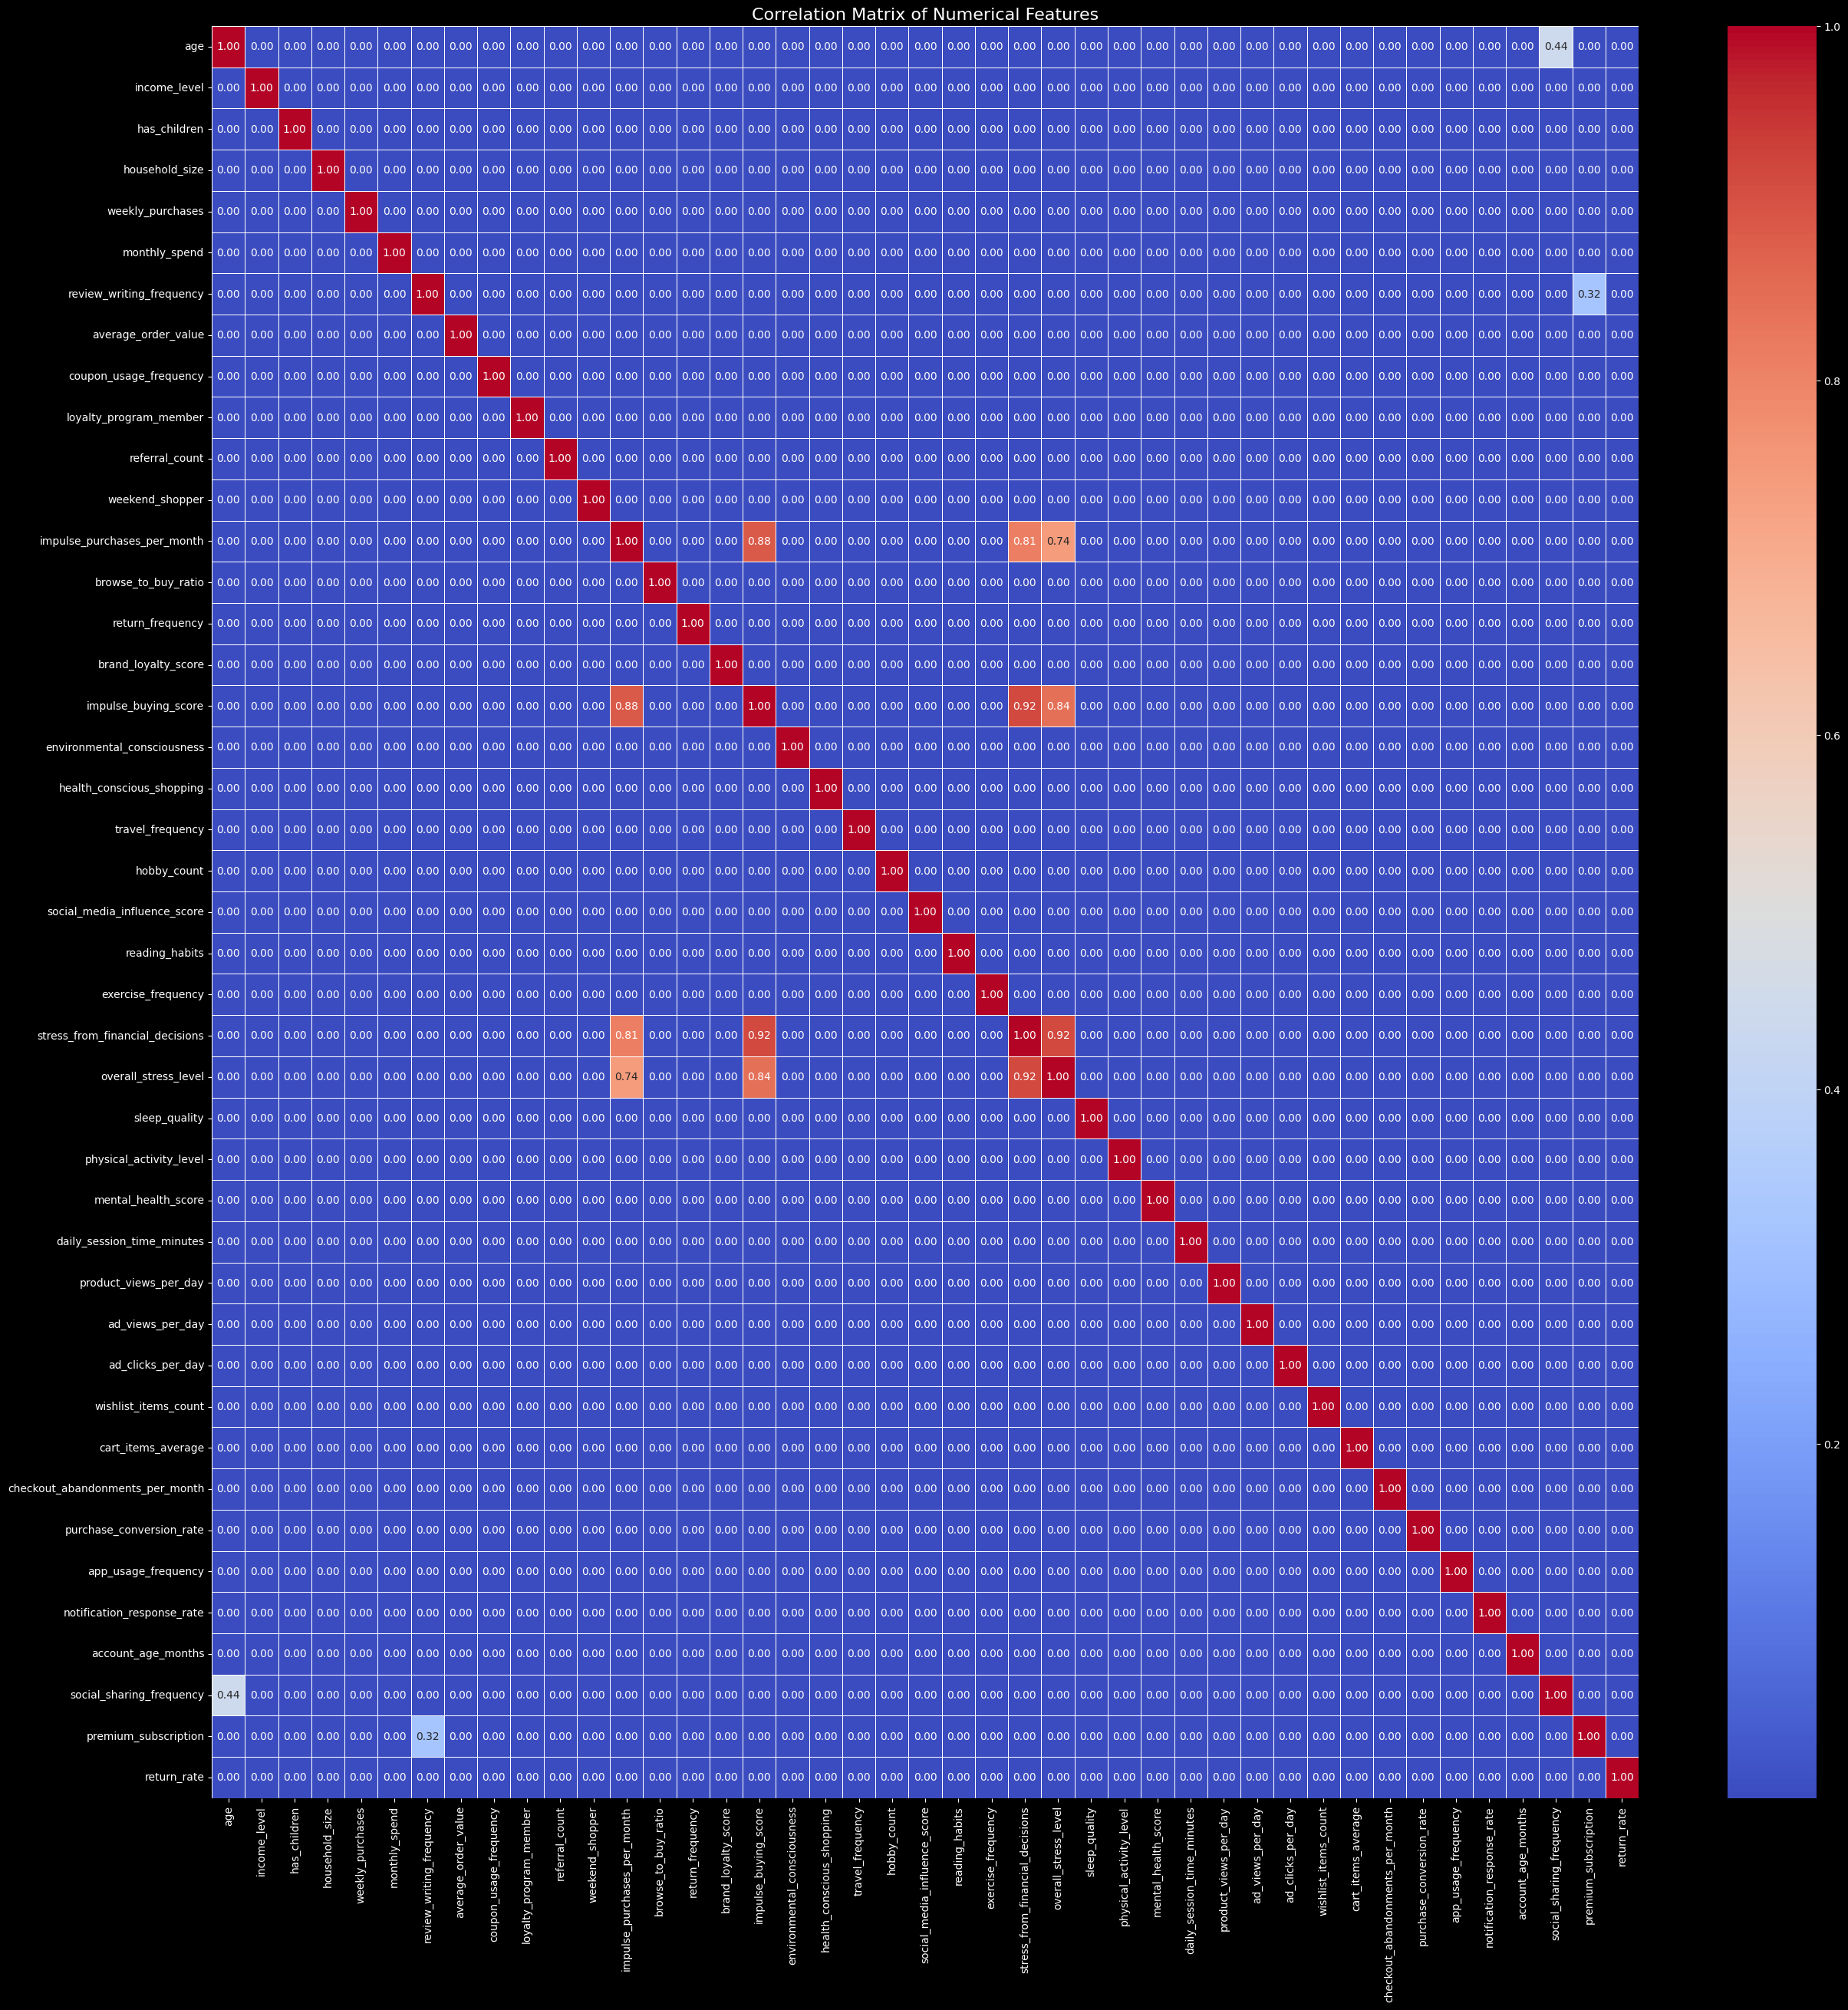
\includegraphics[width=\textwidth,height=0.82\textheight,keepaspectratio]{03_numerical_correlation.png}
\caption{Correlation matrix for numerical features.}
\end{figure}

The notebook then keeps numerical features with non-trivial correlation to the target and repeats the correlation analysis.

\begin{figure}[H]
\centering
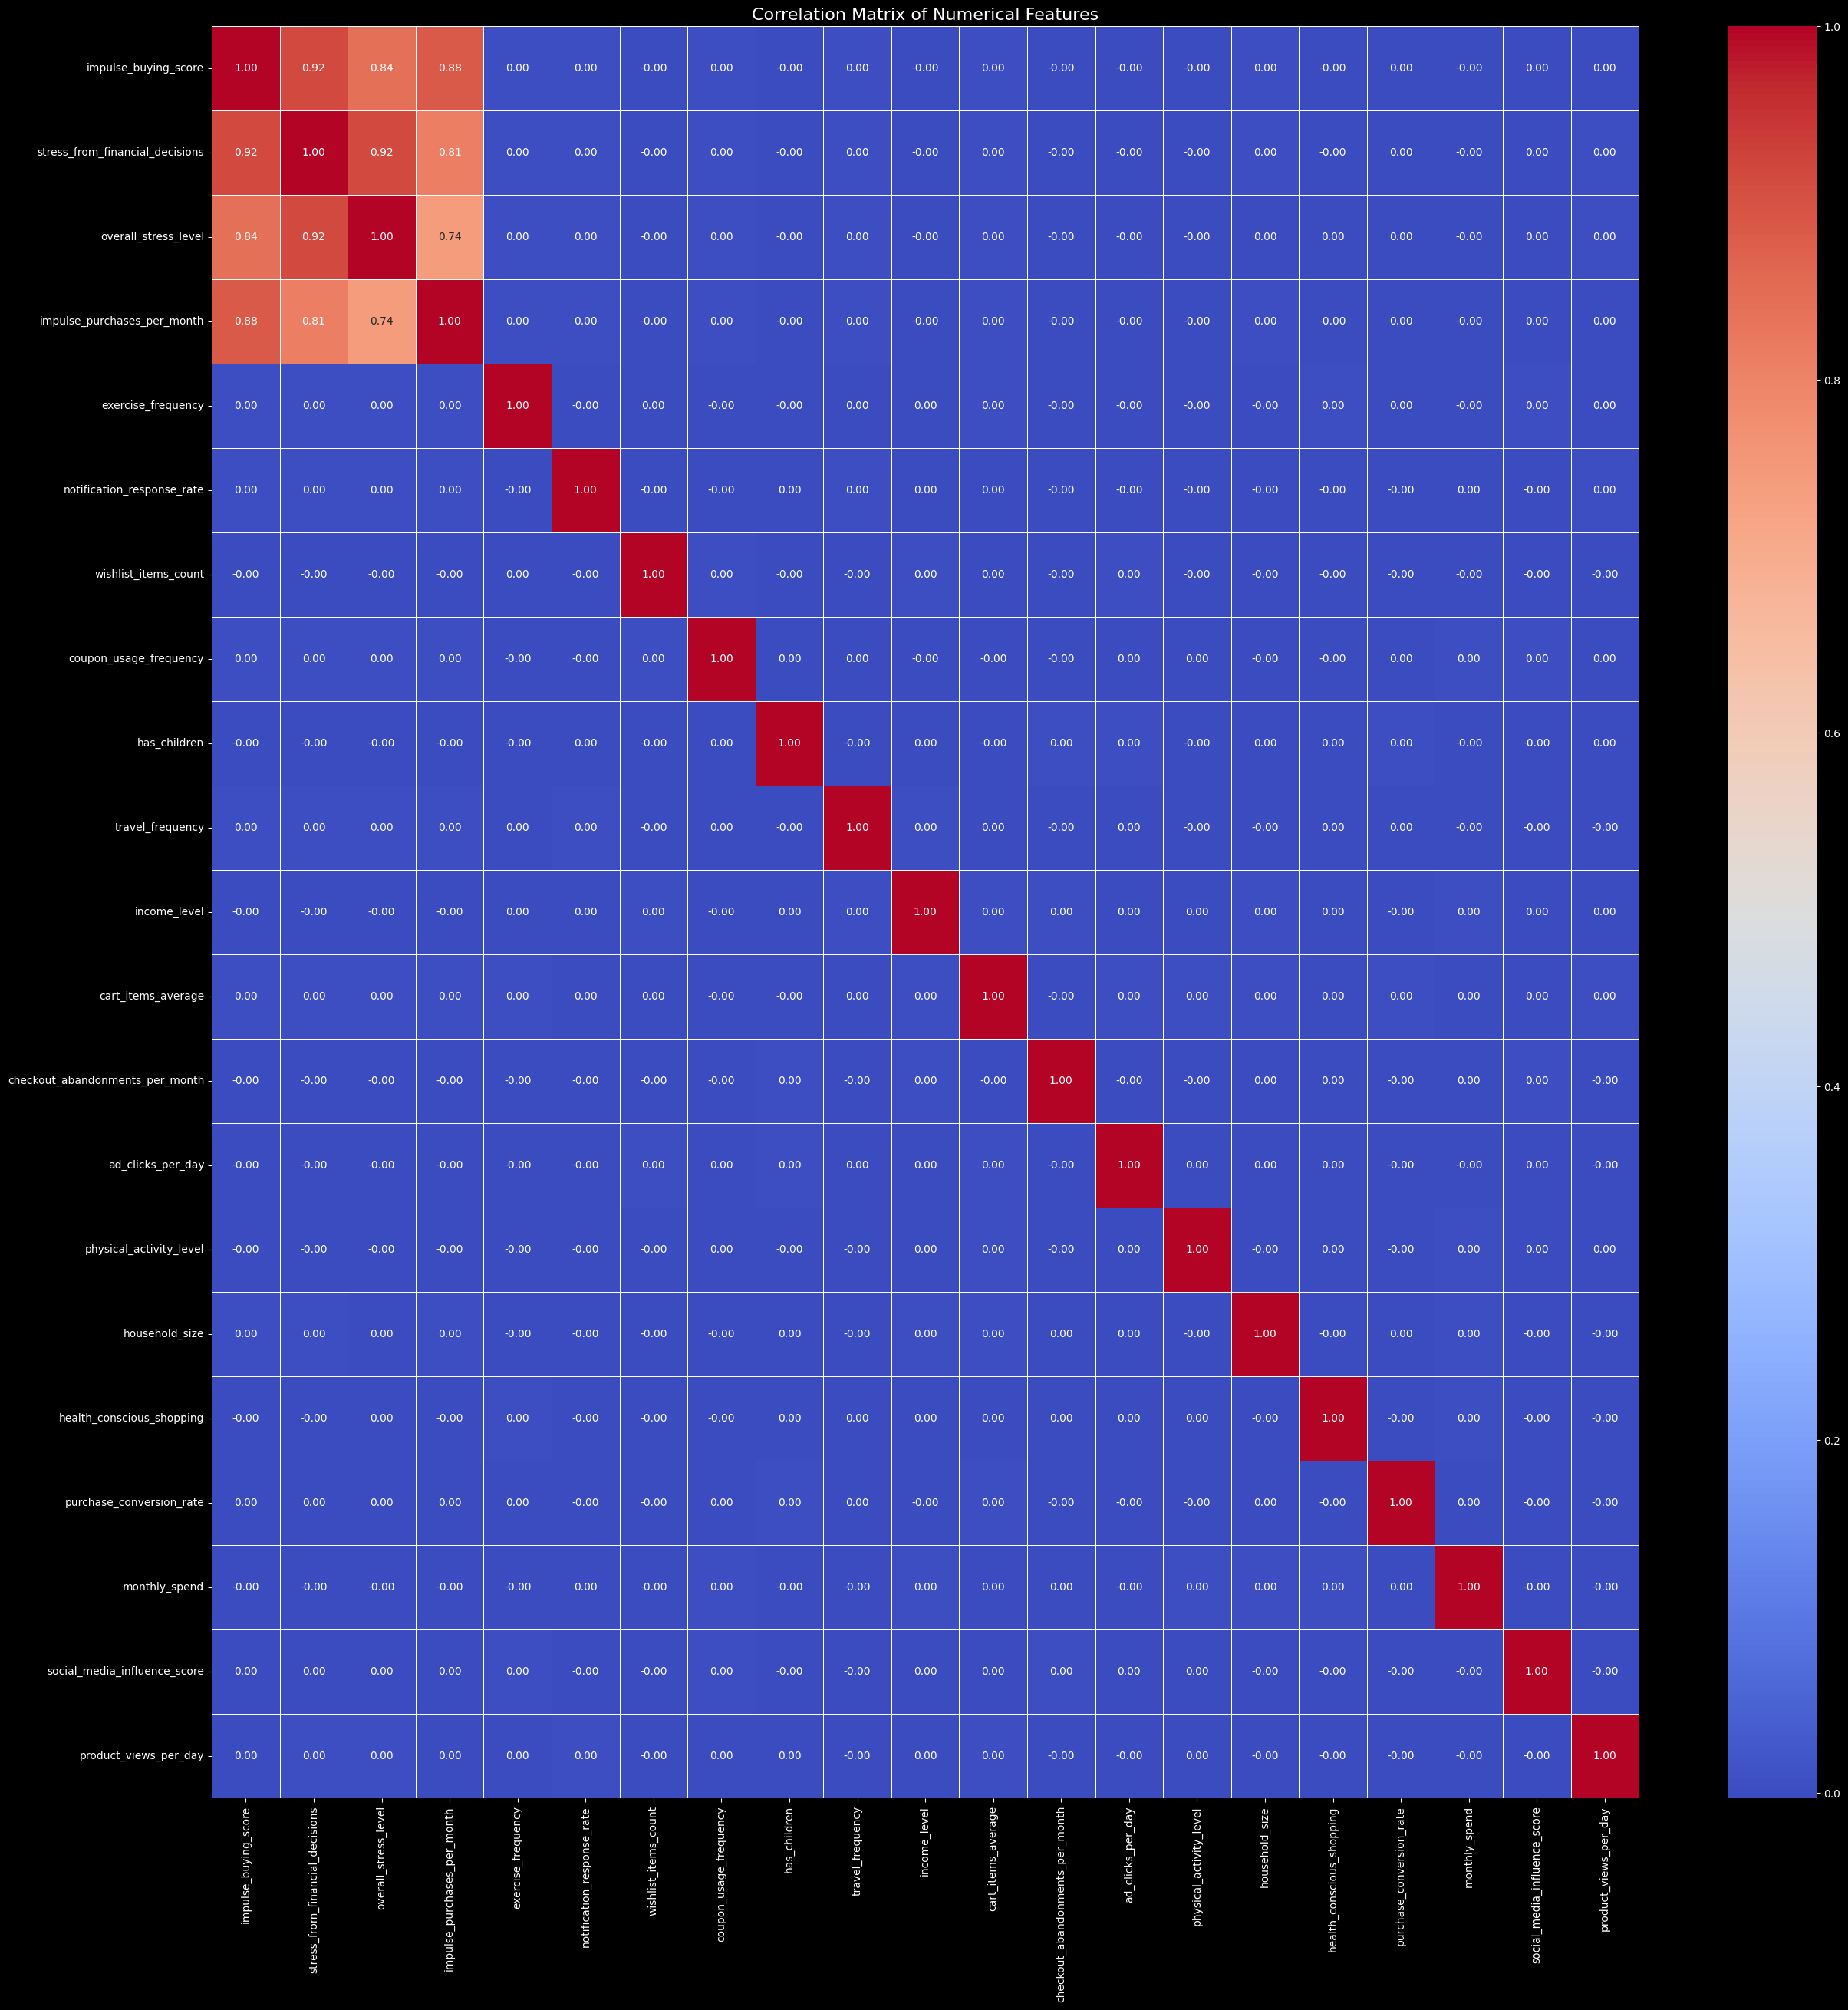
\includegraphics[width=\textwidth,height=0.82\textheight,keepaspectratio]{04_selected_numerical_correlation.png}
\caption{Correlation matrix after removing weakly target-correlated numerical features.}
\end{figure}

\section{Feature Selection}

\subsection{Target-Correlated Numerical Features}

The most target-correlated numerical features found in the preprocessing notebook include:
\begin{center}
\begin{tabular}{p{0.24\textwidth}p{0.66\textwidth}}
\toprule
Group & Features \\
\midrule
Psychological & impulse buying score, financial decision stress, overall stress level \\
Shopping behavior & impulse purchases per month, wishlist item count, cart item average \\
Platform response & notification response rate, ad clicks per day, product views per day \\
Lifestyle & exercise frequency, travel frequency, physical activity level \\
Financial & income level, monthly spend, purchase conversion rate \\
\bottomrule
\end{tabular}
\end{center}

\subsection{Highly Correlated Features}

The notebook detected these strongly correlated feature pairs:
\begin{center}
\begin{tabular}{p{0.72\textwidth}r}
\toprule
Feature Pair & Correlation \\
\midrule
impulse buying score and financial decision stress & 0.92 \\
impulse buying score and impulse purchases per month & 0.88 \\
financial decision stress and overall stress level & 0.92 \\
\bottomrule
\end{tabular}
\end{center}

To reduce redundancy, the lower target-correlated feature from each highly correlated pair is dropped. The recorded columns dropped due to high correlation were:
\begin{verbatim}
overall_stress_level,
stress_from_financial_decisions,
impulse_purchases_per_month
\end{verbatim}

\section{Preprocessing}

\subsection{Ordinal Encoding}

Two categorical features have a natural order and are encoded manually:
\begin{center}
\begin{tabular}{p{0.25\textwidth}p{0.65\textwidth}}
\toprule
Feature & Encoding \\
\midrule
education level & High School = 0, Associate Degree = 1, Bachelor = 2, Master = 3, PhD = 4 \\
budgeting style & Loose = 0, Moderate = 1, Strict = 2 \\
\bottomrule
\end{tabular}
\end{center}

\subsection{Scaling and Binary Encoding}

The selected numerical columns are standardized with \texttt{StandardScaler}. Remaining nominal categorical columns are encoded with \texttt{BinaryEncoder}. These transformations are combined in a \texttt{ColumnTransformer}.

The final preprocessing bundle stores:
\begin{itemize}
  \item the fitted feature preprocessor;
  \item the target scaler for regression;
  \item the selected feature list.
\end{itemize}

The preprocessed arrays are saved as:
\begin{verbatim}
X_train.npy, X_val.npy, X_test.npy
y_train_scaled.npy, y_val_scaled.npy, y_test_scaled.npy
y_train_classified.npy, y_val_classified.npy, y_test_classified.npy
\end{verbatim}

\section{MapReduce-Based Logistic Regression}

The custom logistic regression implementation lives in \texttt{logistic\_regression.py}. It is implemented with NumPy and Spark RDD partitions rather than using scikit-learn's built-in logistic regression.

\subsection{Ordinal Threshold Strategy}

Because the classes are ordered, the model trains two binary logistic regression models:
\begin{center}
\begin{tabular}{cl}
\toprule
Threshold Model & Binary Question \\
\midrule
$y \geq 1$ & Is this shopper at least medium abandonment? \\
$y \geq 2$ & Is this shopper high abandonment? \\
\bottomrule
\end{tabular}
\end{center}

After training, the two probabilities are converted back into three class probabilities:
\[
P(y=0) = 1 - P(y \geq 1),
\]
\[
P(y=1) = P(y \geq 1) - P(y \geq 2),
\]
\[
P(y=2) = P(y \geq 2).
\]

The predicted class is the class with the highest probability.

\subsection{Training}

The notebook starts a local Spark session and splits the training set into 2 to 8 partitions:
\begin{verbatim}
num_partitions = max(2, min(8, sc.defaultParallelism))
\end{verbatim}

Each partition computes its local gradient, loss, and row count. Spark then reduces these partial results into global totals. Each threshold model is trained for 25 epochs using full-batch gradient descent.

The binary cross-entropy loss used for each threshold is:
\[
L = - \left[y \log(p) + (1-y)\log(1-p)\right].
\]

The gradient update is:
\[
\nabla = \frac{1}{N}\sum_i (p_i - y_i)x_i + \lambda w.
\]

In the code this appears as:
\begin{verbatim}
gradient = (grad_sum / count) + reg * weights
weights -= lr * gradient
\end{verbatim}

The \texttt{reg * weights} term is the L2 regularization gradient, which discourages very large weights.

\subsection{Numerical Stability}

The sigmoid function clips scores to the range $[-30, 30]$:
\begin{verbatim}
z = np.clip(z, -30.0, 30.0)
\end{verbatim}

This avoids overflow in \texttt{np.exp(-z)}. Values above 30 already produce probabilities extremely close to 1, and values below -30 produce probabilities extremely close to 0.

\section{Model Results}

\subsection{Overall Classification Comparison}

\begin{center}
\small
\begin{tabular}{p{0.25\textwidth}rrp{0.31\textwidth}}
\toprule
Model & Accuracy & F1 Score & Main Observation \\
\midrule
KNN & 0.7600 & Not recorded & Useful baseline, but weaker than the learned global classifiers. \\
Ordinal Logistic Regression & 0.8583 & Reported in classification report & Strong custom Spark/MapReduce model that respects class order. \\
Decision Tree & 0.8654 & 0.8664 & Strong interpretable tree baseline. \\
Random Forest & 0.8663 & 0.8674 & Best recorded classifier. \\
Linear SVM / SVC & 0.6600 & 0.5254 & Weakest recorded classifier. \\
\bottomrule
\end{tabular}
\end{center}
\normalsize

Random Forest achieved the best recorded accuracy and F1 score, followed closely by Decision Tree and ordinal logistic regression. Linear SVM performed worst among the recorded classifiers. This means the relationship between shopper features and abandonment class is not captured well by a simple linear separating boundary, while tree-based models can capture non-linear feature interactions.

\subsection{KNN Baseline}

The KNN notebook experiment tested several values of $k$:
\[
k \in \{9, 11, 13, 15, 17\}.
\]

The final selected KNN model used:
\begin{verbatim}
n_neighbors = 17
\end{verbatim}

The recorded results were:
\begin{center}
\begin{tabular}{lrr}
\toprule
Split & Rows & Accuracy \\
\midrule
Training & 800000 & 0.81 \\
Validation & 100000 & 0.76 \\
\bottomrule
\end{tabular}
\end{center}

KNN is easy to understand because it predicts using nearby examples. However, it is expensive on a dataset with 800000 training rows because prediction requires comparing a new shopper to many stored shoppers. This makes it less attractive for production deployment than tree-based models or logistic regression.

\subsection{Ordinal Logistic Regression Details}

The ordinal logistic regression model produced:
\begin{center}
\begin{tabular}{lrrr}
\toprule
Split & Accuracy & Class 0 F1 & Class 2 F1 \\
\midrule
Validation & 0.8599 & 0.9062 & 0.8767 \\
Test & 0.8583 & 0.9053 & 0.8748 \\
\bottomrule
\end{tabular}
\end{center}

The test confusion matrix was:
\begin{center}
\begin{tabular}{lrrr}
\toprule
True / Predicted & 0 & 1 & 2 \\
\midrule
0 & 34310 & 3722 & 0 \\
1 & 3453 & 27082 & 3398 \\
2 & 0 & 3598 & 24437 \\
\bottomrule
\end{tabular}
\end{center}

The structure of this confusion matrix makes sense for an ordinal model: most mistakes are between neighboring classes. Class 0 is not directly confused with class 2 in the recorded test output.

\subsection{Decision Tree and Random Forest}

The Spark tree models were trained on the preprocessed feature matrix. The Decision Tree used:
\begin{verbatim}
DecisionTreeClassifier(
    labelCol="label",
    featuresCol="features",
    maxDepth=10,
    maxBins=64,
    impurity="gini"
)
\end{verbatim}

The Random Forest used a sampled training subset and multiple trees:
\begin{verbatim}
RandomForestClassifier(
    numTrees=25,
    maxDepth=8,
    maxBins=32,
    featureSubsetStrategy="sqrt",
    subsamplingRate=0.8,
    seed=42
)
\end{verbatim}

\begin{center}
\begin{tabular}{lrr}
\toprule
Model & Validation Accuracy & Weighted F1 \\
\midrule
Decision Tree & 0.8654 & 0.8664 \\
Random Forest & 0.8663 & 0.8674 \\
\bottomrule
\end{tabular}
\end{center}

The tree models slightly outperformed ordinal logistic regression. This is expected because tree models can split on feature thresholds and combine variables in non-linear ways. Random Forest improves stability by averaging many trees, which explains why it produced the strongest recorded score.

\subsection{Linear SVM / SVC}

The Linear SVM experiment used Spark's \texttt{LinearSVC} inside a \texttt{OneVsRest} wrapper:
\begin{verbatim}
LinearSVC(maxIter=100, regParam=0.1)
\end{verbatim}

Because \texttt{LinearSVC} is binary, \texttt{OneVsRest} trains one binary classifier per class and then chooses the class with the strongest score. The recorded validation result was:
\begin{center}
\begin{tabular}{lrr}
\toprule
Model & Accuracy & Weighted F1 \\
\midrule
One-vs-Rest Linear SVM & 0.6600 & 0.5254 \\
\bottomrule
\end{tabular}
\end{center}

This model performed poorly compared with the other classifiers. A likely reason is that the three abandonment groups are not cleanly separable by linear boundaries in the transformed feature space. The result is still useful because it shows that the project compared different modeling assumptions rather than relying on one method.

\subsection{Regression Model}

The MapReduce linear regression baseline predicts the scaled continuous cart abandonment rate. Its recorded errors were:
\begin{center}
\begin{tabular}{lr}
\toprule
Split & MSE \\
\midrule
Validation & 0.080565 \\
Test & 0.080430 \\
\bottomrule
\end{tabular}
\end{center}

\section{Shopper Segmentation}

The project also applies K-Means clustering to the preprocessed feature matrix to create shopper behavior segments. The notebook evaluates multiple values of $k$ using inertia and silhouette score. The selected number of clusters is:
\[
k = 2.
\]

The K-Means experiment used the transformed training matrix:
\[
X_{\text{train}} \in \mathbb{R}^{800000 \times 57}.
\]

For model selection, the notebook sampled 100000 rows and evaluated $k$ from 2 to 8.

\begin{center}
\begin{tabular}{rrr}
\toprule
$k$ & Inertia & Silhouette \\
\midrule
2 & 2739395.00 & 0.035334 \\
3 & 2693839.25 & 0.025770 \\
4 & 2656088.00 & 0.022683 \\
5 & 2616208.00 & 0.027660 \\
6 & 2594059.25 & 0.026000 \\
7 & 2579117.50 & 0.025884 \\
8 & 2564881.50 & 0.021841 \\
\bottomrule
\end{tabular}
\end{center}

\begin{figure}[H]
\centering
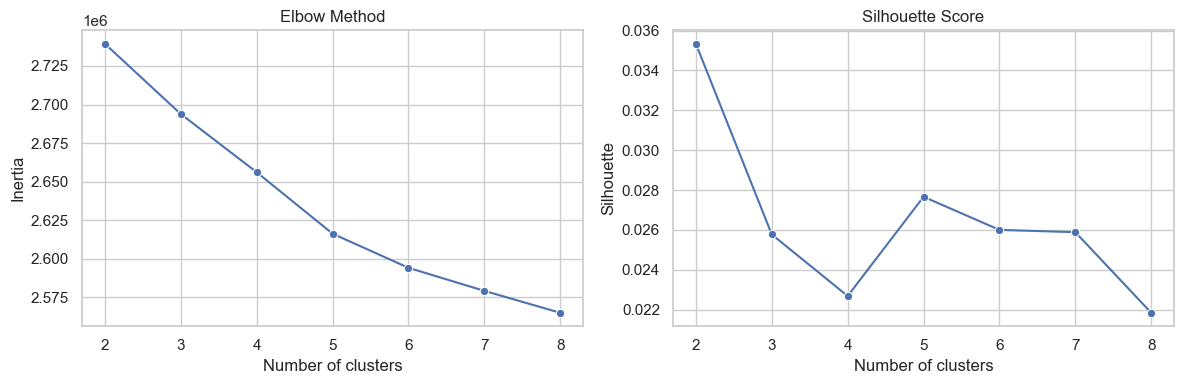
\includegraphics[width=0.92\textwidth]{05_kmeans_elbow_silhouette.png}
\caption{K-Means inertia and silhouette diagnostics from the models notebook.}
\end{figure}

Although inertia decreases as $k$ increases, the silhouette score is highest at $k=2$. The notebook therefore selected two shopper segments.

\begin{center}
\begin{tabular}{lrr}
\toprule
Segment & User Count & Percent of Users \\
\midrule
0 & 399601 & 49.95\% \\
1 & 400399 & 50.05\% \\
\bottomrule
\end{tabular}
\end{center}

The spend-class mix is almost identical across the two clusters:
\begin{center}
\begin{tabular}{lrrr}
\toprule
Segment & Class 0 & Class 1 & Class 2 \\
\midrule
0 & 38.22\% & 33.88\% & 27.90\% \\
1 & 38.09\% & 33.96\% & 27.95\% \\
\bottomrule
\end{tabular}
\end{center}

This means the clusters are not simply low-, medium-, and high-abandonment groups. Instead, K-Means is describing different shopper profiles in the input features.

\begin{figure}[H]
\centering
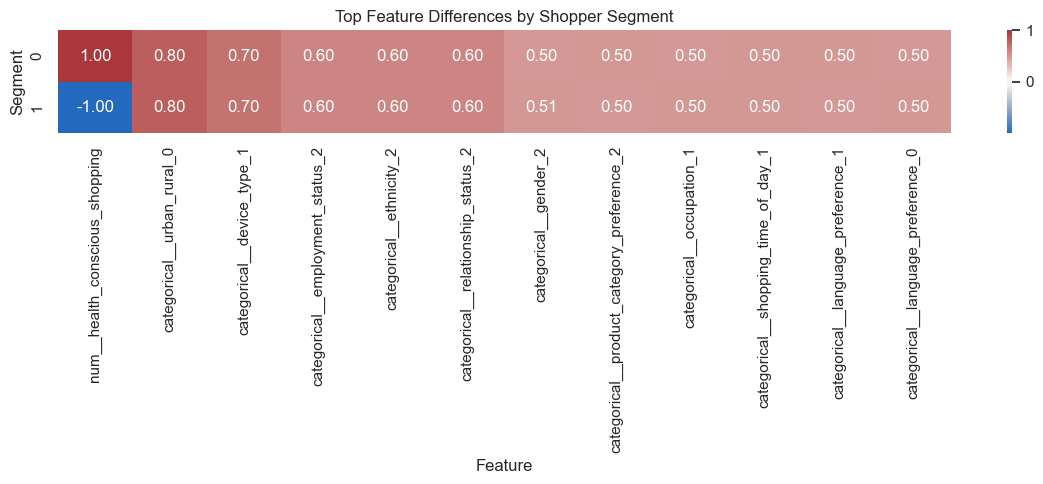
\includegraphics[width=0.95\textwidth]{06_kmeans_segment_profile_heatmap.png}
\caption{Top feature differences between the two shopper segments.}
\end{figure}

The heatmap shows which transformed features are above or below average for each segment. One clear difference recorded in the notebook is that health-conscious shopping is higher in segment 0 and lower in segment 1. Segment 1 is also associated with stronger values for some encoded categorical features, such as the urban/rural encoded variables.

\begin{figure}[H]
\centering
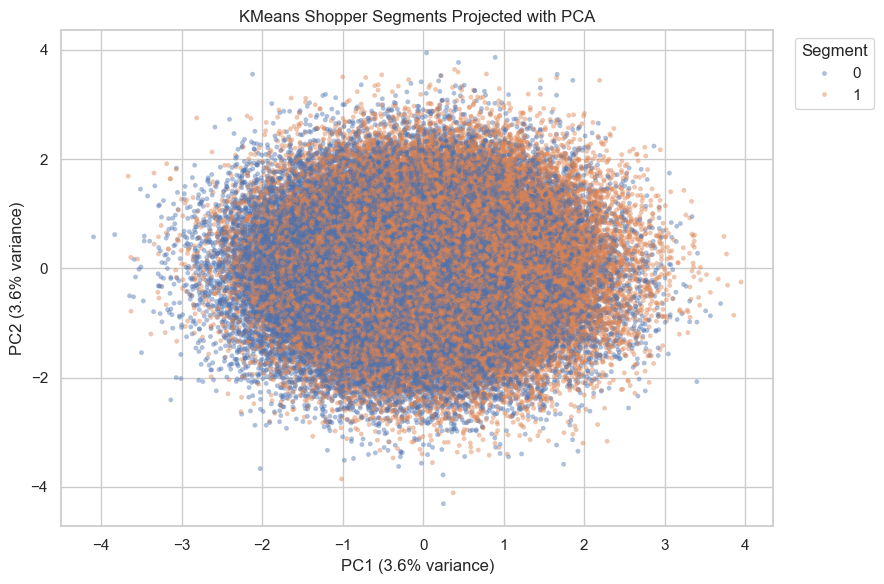
\includegraphics[width=0.92\textwidth]{07_kmeans_pca_projection.png}
\caption{Two K-Means shopper segments projected into two PCA dimensions.}
\end{figure}

The PCA plot gives a two-dimensional view of the clusters. It is not the space where K-Means was trained, but it helps visually inspect whether the two segments form distinguishable regions after dimensionality reduction.

\section{Deployment}

The deployment module wraps the trained artifacts behind a model service. It supports classifier names such as:
\begin{verbatim}
knn
logistic_regression
ordinal_logistic
ordinal_logistic_threshold_weights
\end{verbatim}

For ordinal logistic regression, the service:
\begin{itemize}
  \item prepares and transforms the input data;
  \item adds the bias column;
  \item computes $P(y \geq 1)$ and $P(y \geq 2)$;
  \item converts threshold probabilities into class probabilities;
  \item returns the class with maximum probability.
\end{itemize}

\section{Reproducibility}

The report can be rebuilt from the \texttt{docs} directory:
\begin{verbatim}
make pdf
\end{verbatim}

This command first runs:
\begin{verbatim}
python3 generate_preprocessing_plots.py
\end{verbatim}

and then compiles the LaTeX report with \texttt{pdflatex}. If the original Kaggle CSV is placed in the repository root as:
\begin{verbatim}
e_commerce_shopper_behaviour_and_lifestyle.csv
\end{verbatim}

the plot script regenerates the preprocessing figures from data. Otherwise it extracts the exact saved plot outputs from \texttt{preprocessing.ipynb}.

\section{Limitations and Next Steps}

\begin{itemize}
  \item The original CSV is not committed in this repository, so the local report build currently relies on embedded notebook plot outputs unless the CSV is provided.
  \item KNN is expensive for very large datasets and is less practical for production inference than tree-based models or logistic regression.
  \item The custom logistic regression is useful for demonstrating MapReduce training, but Random Forest achieved slightly better metrics.
  \item Future work should add clearer model artifact versioning and a single end-to-end training command.
  \item The report could be extended with deployment API examples and more detailed K-Means cluster profiles.
\end{itemize}

\section{Conclusion}

The project builds a complete shopper behavior pipeline from raw data to preprocessing, visualization, model training, segmentation, and deployment. The most important predictors are related to impulsive shopping, financial stress, notification response, wishlist behavior, and conversion behavior. Random Forest produced the strongest recorded classification result, while the custom ordinal logistic regression remains valuable because it uses the ordered nature of the target classes and demonstrates distributed gradient computation with Spark.

\end{document}
